\begin{abstract}
    \small

TODO

\end{abstract}

\begin{otherlanguage}{ngerman}
    \begin{abstract}
        \small

Eines der größten Probleme von E-Mail Kommunikation ist, dass diese fast ausschließlich unverschlüsselt abläuft.
Die Erstellung von E-Mail-Verschlüsselungs Zertifikaten ist meißtend nur schlecht in Unternehmensabläufe eingebunden und
daher für Nutzer nur schlecht zugänglich.
Da alle Vorraussetzungen für starke Verschlüsselung, zumindest bei interner E-Mail Kommunikation gegeben sind, sollte
diese standardmäßig aktiviert sein.
Um dies zu ermöglichen, implementieren wir in unserer Arbeit ein Zertifikatsverwaltungssystem, das stark in bestehende
Unternehmensabläufe integriert ist.

Die hauptsächlichen Funktionen, die in dieser Arbeit erstellt wurden sind:
\begin{itemize}
    \item Den schon vorhandenen Code zur Zertifikatsverwaltung für schon existierende Infrastruktur zu portieren
    \item Die Nutzer- und Zertifikatsverwaltung in bestehende Verzeichnisdienste zu integrieren
    \item Die Benutzerseitigen Prozesse weitestgehend zu automatisieren
\end{itemize}

Das Resultat unserer Arbeit is ein funktionierendes, experimentelles Web basiertes Zertifikatsverwaltungssystem, das in
der Lage ist automatisch Zertifikate für Benutzer der TUM zu erzeugen.
Obwohl für den allgemeinen Einsatz noch eine vertrauenswürdige Zertifizierungsstelle fehlt, fuktioniert das System
bereits mit selbst signierten Zertifikaten und erlaubt es Nutzern einfacher E-Mails zu verschlüsseln.

    \end{abstract}
\end{otherlanguage}

\setcounter{tocdepth}{1}
\tableofcontents
\listoffigures

\startcontent

\chapter{Introduction}\label{ch:introduction}
In 2009 Cavoukian coined the term: \say{Privacy by design}~\cite{cavoukian2009privacy}.
Still today communication in many institutions happens mainly via unencrypted email.
This is very problematic, as personal information of users is exposed to many kinds of misuses.

Designing systems, that employ privacy as a \say{critical enabler of trust and freedoms in our present-day information
society}~\cite{cavoukian2009privacy} should be in the focus of any respected institution.
At TUM, there are some possibilities to encrypt messages between users, however none of them properly apply Cavoukian's
foundational principles.

Any system, that respects the users privacy should include at last:\\
\textbf{Privacy as the Default Setting}, which means the setting which requires the least user interaction is properly
configured for maximum confidentiality.
Unfortunately, this is not the case for email communication at TUM, since email encryption requires significant
additional work by users, which is caused by bureaucratic acts.
This causes even the most basic service messages to be unencrypted and not authenticated.
This leads to easy attack vectors for impersonation and social engineering.

The system should be \textbf{User-Centric}.
Common criteria for user-centric applications are usability and efficient processes for common use-cases.
TUM's current system also fails those criteria, since all email certificate systems are external and do not integrate
into TUM workflows.
Usability is additionally reduced by a completely foreign design vocabulary and seemingly arbitrary but required
procedures.

Since the current system at TUM fails those principles, the working group \say{secure email} set out to design an email
encryption certificate system, that tries to move the status-quo to a more privacy by default direction.

\section*{Research question}
This interdisciplinary project implements this certificate management system, which integrates better with
organizational workflows.
The system is not not limited TUM, but generalizable to arbitrary organizations by being based on standardized software.
Within this project, we face several problems:
\begin{enumerate}
    \item How should a truly user friendly certificate management system look like?
    \item How can we integrate this system in existing workflows to make it as accessible as possible?
    \item How can we manage certificates in an organization?
    \item What challenges are we facing for certificate based authentication on embedded devices?
\end{enumerate}

For this IDP, we decided to split the problem into frontend and backend.
In this document, we try to solve this problem, with a slight focus on issues in the backend.


\chapter{Related Work}\label{ch:relatedWork}
One of the more recent projects, that provide encryption services is Let's Encrypt.
The Let's Encrypt system provides a way to automatically provide x509 certificates for client to server communication,
e.g.\ for HTTPS\@.
This system works via an Automatic Certificate Management Environment (ACME), which is specified in an IETF standard
working draft~\cite{letsencrypteacme}.

\begin{figure}
    \centering
    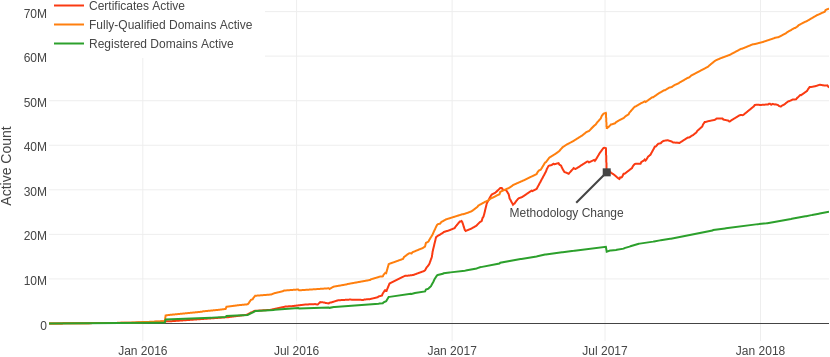
\includegraphics[width=\textwidth]{figures/letsencryptusers.png}
    \caption{Let's Encrypt Growth~\cite{letsencryptstats}}
    \label{fig:letsencrypt}
\end{figure}

This project is already immensely successful, providing over 50 Million active certificates, as of March 2018 (see
Figure~\ref{fig:letsencrypt})

However, this system is not intended for the general population, since the validation challenges aren't end-user
focused, but mostly for webservers.
X.509 certificates, as issued by Let's Encrypt can generally be used for email security with S/MIM\@.
Since this is not the focus of Let's encrypt, they also don't issue certificates, that would be usable for email
encryption.

More work about how email encryption certificates can be managed in a organization has been done by the TUM Secure
Email and User Certification Project~\cite{hauner2016interoperability, jagdish2016certservice, straub2016directoryservice, maier2015multidevice}


\chapter{Public Key Infrastructure}\label{ch:publicKeyInfrastructure}

This chapter explains, how privacy in communication can be achieved and what infrastructure

\section{Public-Key Cryptography}\label{sec:publicKeyCryptography}

"key-management problem with symmetric cryptosystems"

"two different keys - one public and the other private"~\cite{schneier2007applied, diffie1976new}

Public key for encryption, private for decryption.
Private key for signature, public key for signature verification.

To solve the problem of man-in-the-middle attacks, a system of trust is established.
In this system a trusted third party verifies, that the public keys are authentic

\section{Public Key Infrastructure}\label{sec:publicKeyInfrastructure}
please refer to RFC3280

\section{Email Security}\label{sec:emailSecurity}

Security of emails was not a design goal.
Email with it's several protocols is inherently insecure.
Several approaches to secure email, e.g. SMTP over TLS, which only secures traffic but does not provide end-to-end
security.
Truly confidential and authenticated messages only possible with two competing end-to-end cryptographic implementations:
PGP and S/MIME.

\subsection{PGP}\label{subsec:pgp}

Pretty Good Privacy (PGP) was first implemented by Philip Zimmermann in 1991.
Can be used for encryption and signing of data.
See PGP user's guide.

Software support, e.g. in Mozilla Thunderbird via a plugin: Enigmail

OpenPGP, the modern version and de-facto standardized PGP.
Specified in RFC4880.

\subsection{S/MIME}\label{subsec:s/mime}
see RFC5750


\section{Certificates at TUM}\label{sec:certificatesAtTum}

TUM has multiple possible ways of acquiring certificates:

The "Leibniz-Rechenzentrum der Bayerischen Akademie der Wissenschaften" (LRZ in short) offers to sign
certificates~\cite{lrzpki}, which then can be used to secure servers hosted with the LRZ, but also for e-mail security.
The LRZ itself describes the situation as complicated, because of the "many other temporary installed solutions"
("[da] sowohl am LRZ wie auch anderswo provisorische L\"osungen installiert worden sind").

TUM IT-support also offers certification services~\cite{tumZertifikat}.

Additionally, TUMs Faculty of Informatics also runs a registration authority~\cite{inTumCertificates}.

All three of those certification solutions are based on the CA of the Deutsches Forschungsnetz (DFN)~\cite{dfnPki}.
So, in theory any one certification method should have the same "trust", however the certification requirements and
procedures significantly differ.
Furthermore, the process of generating public keys is not handled very well: LRZ provides a guide to generate keys with
the \lstinline{openssl} command line utilities, which disqualifies a lot of the users from using the RA\@.
The Faculty of Informatics generates the keys for their users and stores them secured with a RA generated passphrase.
This fails one of the basic requirements of public-key cryptography, that only the user should ever have access to the
private key.
TUM-IT uses the DFNs webinterface to generate keys, which generates the keys in the users browser and encrypts them with
a user provided passphrase.
This process is a really good compromise between the ability of a layman to generate keys, while not breaking
cryptography guidelines.
However, this webinterface is not very accessible, especially on mobile devices and additionally completely separated
from TUM infrastructure, such that basic integration within TUM workflows or many quality-of-life improvements can't be
made.



\chapter{Design}\label{ch:design}

In this chapter we describe the approach and design of the of the implemented solution.
First and foremost, a automatic certification process should avoid user interaction whenever possible.

\begin{figure}
    \centering
    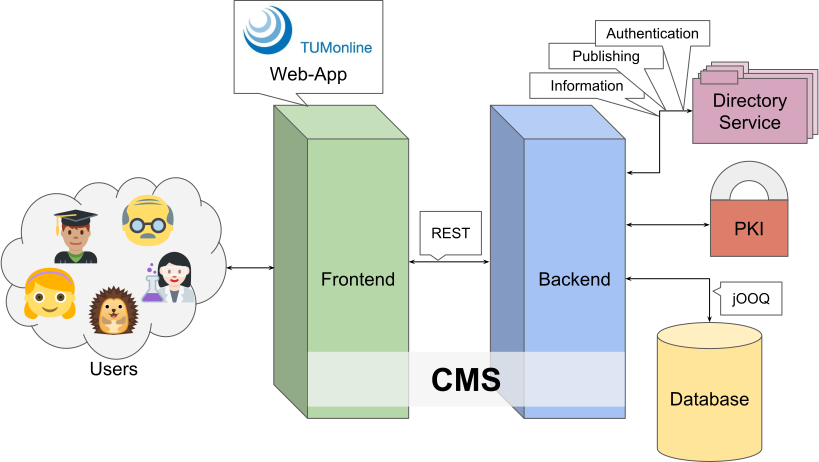
\includegraphics[width=.8\textwidth]{figures/systemArchitecture.pdf} % TODO see jagdish2016certservice
    \caption{Architecture of the certificate management system}
    \label{fig:systemArchitecture}
\end{figure}

The basic architecture is displayed in Figure~\ref{fig:systemArchitecture}.
% TODO: the basic architecture, similar to the one proposed by jagdish2016certservice is shown in Figure~, however the final architecture has
% some differences. The identity management, authentication and keyserver / public key publishment components are all
% separate in his design, in reality most systems handle all this via a single directory service.
In our approach, a web application handles the user interaction in a nice and user friendly way.
This webapp can be provided by familiar user interfaces, such as TUMonline in case of our university.
The app then in turn communicates with a certification management system as backend, that can handle the certification
components.

\section{User Centric features}\label{sec:userDetails}
Certificates require some fields regarding information of the user.
Since most of this information is readily available in organizations user identity management systems, this information
should be used to reduce the interaction the user needs to have with the system.

This identity management can also be used to authenticate the user.
Since most institutions have already verified users identities, those systems can be used as basis of trust.

However, providing a secure way to backup certificates of users is essential to provide a good user experience.

\section{Integration Into Existing Systems}\label{sec:integrationIntoExistingSystems}
User friendliness is not only a design goal of the frontend, but also the backend APIs, that are documented and can be
used intuitively.
Reduction of setup, deployment and development complexity, results in a intuitive for administrators and future
extensions of the system.

Another important factor is the usage of industry standard tools, such as Java enterprise application.
Java enterprise servers are often already available in organizations, but can also easily be set up separately.
Different databases in organizations, provide abstraction from concrete database.

To implement a generic database connection we decided to use an Object Relational Mapper (ORM), that works with any
database an organization wishes to use.
Previously only MySQL was supported, a more generalized approach would be better, e.g.\ to store data in an Oracle
database, such as TUM uses for its TUMonline.

Furthermore, mismatches between database schema and Java objects are only detected during runtime, which increases
testing overhead.
This can be statically checked at compile time, which should decrease bugs and increase developer productivity

\section{Compatibility With Embedded Devices}\label{sec:compatibilityWithEmbeddedDevices}
With the rise of the Internet of Things (IoT), many appliances have a need to communicate with users and each other.
To also provide certificates to those devices, we envision complete hands-off provisioning of certificates on embedded
devices.
To enable those applications, we design our solution to be fully scriptable, complete with generation and distribution
of certificates.
This essentially boils down to providing an API, which can be universally used.
Such APIs are commonly designed as Representational State Transfer (REST) systems, which we decided to use.

\section{Certificate Exchange}\label{sec:certificateExchange}
One of the main features for PKI (c.f.~\ref{sec:publicKeyInfrastructure}), the Certificate Repository also needs to be
added, such that certificates can be published in a more generic way.
To implement such a repository, there are several different methods, as detailed by
Hauner~\cite{hauner2016interoperability}:
One possibility would be to publish the certificates via the Lightweight Directory Access Protocol (LDAP).
The specification in RFC4523~\cite{RFC4523} defines the \lstinline{userCertificate} field for X.509 Certificates.

An alternative would be DNS-Based Authentication of Named Entities (DANE), as defined in RFC8162~\cite{RFC8162} via the
SMIMEA DNS record.
Similar to that approach, OpenPGP certificates can also be published using DANE, as defined in RFC7929~\cite{RFC7929}.
However in this work, we will only concentrate on on X.509 certificates, but lay the foundations to future extensions
to support OpenPGP

Since there are two competing options in this case, we decided to only concentrate on the most widespread and accessible
option in organizations: LDAP\@.
LDAP servers are almost universally available, since most user authentication systems are based on it, most famously
Microsoft's Active Directory.


\chapter{Implementation}\label{ch:implementation}
In this chapter, we describe the process of applying the design as described in Chapter~\ref{ch:design} to the
Certificate Management System.

\section{Exising Prototype}\label{sec:exisingPrototype}
Dr.\ Wachs et al.\ already implemented a prototype, that can be used to issue and manage certificates.
This system can be used as basis of our work, however several key features are still lacking:

After analyzing the prototype, it seemed overly complex and overly modularized.
Several abstractions don't make sense, i.e.\ it was designed to support different so-called "Runtime Abstraction
Layers", while none of that abstraction was needed.
Furthermore, the project was on first sight modularized with several "common" modules, which turned out to be tightly
coupled into the whole system.
This made things worse than no modularization at all, since related classes were distributed between modules and
functionality was duplicated between modules.

Also the deployment of the software was rather fragile and consisting of a combination of bash and maven files and
separate database configuration instructions, which needed to be executed in the right order.
This resulted in a scary deployment process, which resulted in a virtual machine, which was updated every once in a
while.
This is obviously a bad idea, since any \say{Runtime Abstraction} prior to that machine was rendered useless.

Furthermore, when looking at the Java code, no clear lines of input validation or error propagation were visible.
Almost every class had their own null pointer checks, and returning null themselves in error cases and only logging the
error message.
This resulted in the vast majority of unit tests being dedicated to nullability checks.

Lastly, almost all user management features were not included in the overall design of the system, which already
struggled under its own complexity, while lacking some of the most basic features.
% TODO: missing features as described earlier

\section{Complexity Reduction}\label{sec:complexityReduction}
% TODO
No RAL, only a single Spring Boot Application

Bundled competences with reduced modularization: Certificate Management System and REST-API and completely separate Frontend module

% TODO: cite https://en.wikipedia.org/wiki/Design_by_contract#cite_note-3
Applied the design by contract methodology, to reduce the overall \lstinline{null} handling.
Around 50\% of all tests were focused on handling nullable types, ensuring null input produces null output and
generally, that errors result in null values.
However, since for almost all cases, null values indicate input errors and should not propagate throughout the entire
system.
We therefore eliminated most usages of null and used Java Annotations, supporting nullability contracts
(\lstinline{@Nullable} or \lstinline{@NotNull}).
This way, the overall number of paths through the code is reduced significantly reduced and all input verification is
actually handled at the time of input, which additionally provides much better error messages.

Additionally, many errors caused by violated assertions, i.e.\ programming errors, now cause exceptions.
Exceptions have the advantage to fail hard, instead of generating propagating null values and actually be logged,
instead of being swallowed by generic null handling code.

\section{Deployment With Gradle}\label{sec:deploymentWithGradle}
% TODO: proof read
The previous build automation system was based on Apache Maven, combined with Makefiles and Bash scripts.
This made the development environment non-portable, but only buildable on Linux and resulted in slow build times and
inflexible extensibility.
Because of this system, multiple separate configuration scripts needed to be executed in the right order, despite having
a build system.
An integration of modern web development frameworks was also not easily possible in this setup, but would result in
additional manual configuration effort.
This should obviously be handled via the build system. % TODO
A more suited and modern alternative is Gradle, which we used to reduce the need for separate scripts, since Gradle can
be used to perform arbitrary tasks using the Apache Groovy language.

Updating dependencies should be easy, especially for a security-critical application like ours.
More than 25 different third-party libraries used for this project.
Updating those dependencies is necessary for security updates, especially in a security oriented application, handling
sensitive information of users and responsible to secure certificates.

Outdated dependencies can be detected via the \say{gradle-versions-plugin}, which displays the newest available versions
from open-source repositories.
% TODO: an example, how outdated libraries are reported is shown in the listing below

\begin{lstlisting}
$ gradle dependencyUpdates
------------------------------------------------------------
: Project Dependency Updates (report to plain text file)
------------------------------------------------------------

The following dependencies are using the latest integration version:
- org.apache.directory.server:apacheds-all:2.0.0-M24
- dfncert:client:1.9.1
- io.jsonwebtoken:jjwt:0.9.0
[...]

The following dependencies have later milestone versions:
- org.bouncycastle:bcmail-jdk15on [1.56 -> 1.59]
- org.bouncycastle:bcpg-jdk15on [1.56 -> 1.59]
- org.mariadb.jdbc:mariadb-java-client [2.2.3 -> 2.2.5]
[...]
\end{lstlisting}

% TODO: This enables periodic builds, e.g. on a continous integration server to auotmatically detect security updates

While handling the dependency updates, we noticed problems with updating individual dependencies, since the dependencies
have internal dependencies themselves, commonly described as \say{Dependency Hell}: %https://en.wikipedia.org/wiki/Dependency_hell

Especially time consuming and frustrating, since mismatched versions of the Spring Framework and dependent dependencies
can lead to a \lstinline{ClassNotFoundException} at runtime.
This is inherently due to Javas implementation of lazily loading classes~\cite{gosling2014java}.

Our implementation solves this, by specifying version numbers globally, which removes the possibility of \say{missing} to
update one dependent version.
This couples compatible versions of the Spring Framework and Log4J together which should automatically keep the versions
compatible.

\section{Database Versioning And Migrations}\label{sec:databaseVersioningAndMigrations}
While working on the database, we quickly noticed, that the database access needs severe improvement.
Since every change in the database schema resulted in multiple changes in the breakages, all of which only happened at
runtime.
Since none of the existing tests actually verified the database, this only manifested at runtime in hard to debug
crashes.
Also, no good upgrade path is available, since there is no no versioning information available in the database.
The jackhammer method of exporting the whole database and recreating it each time the schema is updated was quickly
discarded.

Instead, we decided to use two industry standard dependencies: jOOQ~\cite{jooq} and flyway~\cite{flyway}

The idea behind jOOQ is static class generation to check matching models at compile time and features an alternative
Domain Specific Language (DSL) to SQL\@.
This idea provides several advantages over classic Java Database Connectivity (JDBC) in combination with raw SQL:
\begin{itemize}
\item Type safety between the database model and the Java application
\item Support for different databases
\item Enterprise support if needed for enterprise databases
\end{itemize}

Flyway provides automate creation of database schema and migration of old data via a gradle task, that can be defined to
automatically apply the correct migrations for the currently deployed version.
This severely reduces the work, that needs to be done when updating the database schema.

All in all, this makes the future development of the application much easier, since for each change to the database,
only a single migration needs to be written.
Subsequently, the matching database models are generated and any mismatches are immediately reported as compiler errors.

\section{Core Features}\label{sec:coreFeatures}
User authentication with LDAP. % TODO
Two different user information approaches:
Or according to Microsoft's Active Directory
Both of which are handled via the LDAP protocol % TODO: cite RFC, summarize auth + user information process

Publishing of certificates can happen via those implementations, i.e.\ publishing of RFC4519~\cite{RFC4519} compliant
exchange between user information.

Automatic approval of certificates.


\chapter{Conclusion}\label{ch:conclusion}
% TODO
Encrypting email is very important.

Enabling users to use encryption requires tight integration into existing workflows.

Requirements for a DFN RA are already met, since all users of TUM's identity management have their identity checked.
Employees need to show their passport when applying for a contract.
Students need to upload a copy of their passport when applying for their program.
The only reasons blocking a roll-out of an automatic and universal certificate management system are or political
nature.

The CMS should also generalize very well to arbitrary organizations, since all required components for integration are
very common.
User authentication in the vast majority of organizations is covered by support for LDAP and Active Directory.
Automatic certificate approval be covered by requirements to check identities, that are usually present for health
insurances, either for employees or at the moment of matriculation.

\chapter{Future Work}\label{ch:futureWork}

Future work includes actual deployment of the system.
% TODO: foundations for a proper long term deployment are there, we only need
This requires acquisition of an actual certificate authority, that is trusted by clients.

Integration into existing infrastructure at TUM also needs to happen, e.g.\ into the CAMPUSonline instance, which should
allow to run JAVA applications

And last but not least the security of the implementations should be independently audited.
Since this system is critical for users trust and freedom, no corners should be cut.
Focus of this work was not the security of the application and questions like, what fields in users certificates are
allowed, were not answered in this work.

\pagestyle{thesischapter}
\cleardoublepage
\setquotestyle{english}
\printbibliography[heading=bibintoc]
